\chapter{The Singular Value Decomposition}
The singular value decomposition (SVD) is a matrix factorization whose computation is a step in many algorithms. Equally important is the use of the SVD for conceptual purposes. Many problems of linear algebra can be better understood if we first ask the question: what if we take the SVD?

\section{A Geometric Observation}
The SVD is motivated by the following geometric fact:
\[
    \text{The image of the unit sphere under any $m \times n$ matrix is a hyperellipse.}
\]
The SVD is applicable to both real and complex matrices. However, in describing the geometric interpretation, we assume as usual that the matrix is real.

%────────────────────────────────────────
\begin{figure}[H]
    \centering
    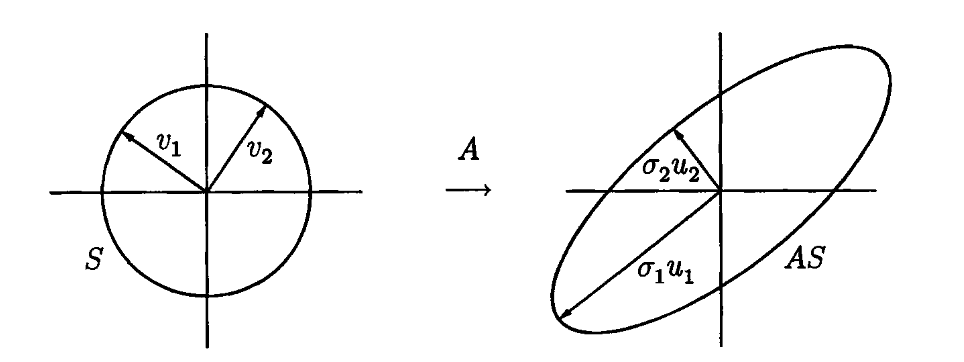
\includegraphics[width=0.8\textwidth]{figures/4-1.png}
    \caption{SVD of a $2\times 2$ matrix}
    \label{fig 4.1}
\end{figure}
%────────────────────────────────────────

Let $S$ be the unit sphere in $\mathbb{R}^n$, and take any $A \in \mathbb{R}^{m \times n}$ with $m \geq n$. For simplicity, suppose for the moment that $A$ has full rank $n$. The image $A S$ is a hyperellipse in $\mathbb{R}^m$. We now define some properties of $A$ in terms of the shape of $A S$. The key ideas are indicated in Figure~\ref{fig 4.1}.

First, we define the $n$ singular values of $A$. These are the lengths of the $n$ principal semiaxes of $A S$, written $\sigma_1, \sigma_2, \ldots, \sigma_n$. It is conventional to assume that the singular values are numbered in descending order, $\sigma_1 \geq \sigma_2 \geq \cdots \geq$ $\sigma_n>0$

Next, we define the $n$ left singular vectors of $A$. These are the unit vectors $\left\{u_1, u_2, \ldots, u_n\right\}$ oriented in the directions of the principal semiaxes of $A S$, numbered to correspond with the singular values. Thus the vector $\sigma_i u_i$ is the $i$ th largest principal semiaxis of $A S$.

Finally, we define the $n$ right singular vectors of $A$. These are the unit vectors $\left\{v_1, v_2, \ldots, v_n\right\} \in S$ that are the preimages of the principal semiaxes of $A S$, numbered so that $A v_j=\sigma_j u_j$.

\section{Reduced SVD} 
We have just mentioned that the equations relating right singular vectors $\left\{v_j\right\}$ and left singular vectors $\left\{u_j\right\}$ can be written
\begin{align*}
A v_j=\sigma_j u_j, \quad 1 \leq j \leq n. 
\end{align*}
More compactly, $A V=\hat{U} \hat{\Sigma}$. In this matrix equation, $\hat{\Sigma}$ is an $n \times n$ diagonal matrix with positive real entries (since $A$ was assumed to have full rank $n$ ), $\hat{U}$ is an $m \times n$ matrix with orthonormal columns, and $V$ is an $n \times n$ matrix with orthonormal columns. Thus $V$ is unitary, and we can multiply on the right by its inverse $V^*$ to obtain
\begin{align*}
A=\hat{U} \hat{\Sigma} V^*
\end{align*}
This factorization of $A$ is called a reduced singular value decomposition, or reduced $S V D$, of $A$. Schematically, it looks like this:
%────────────────────────────────────────
\begin{figure}[H]
    \centering
    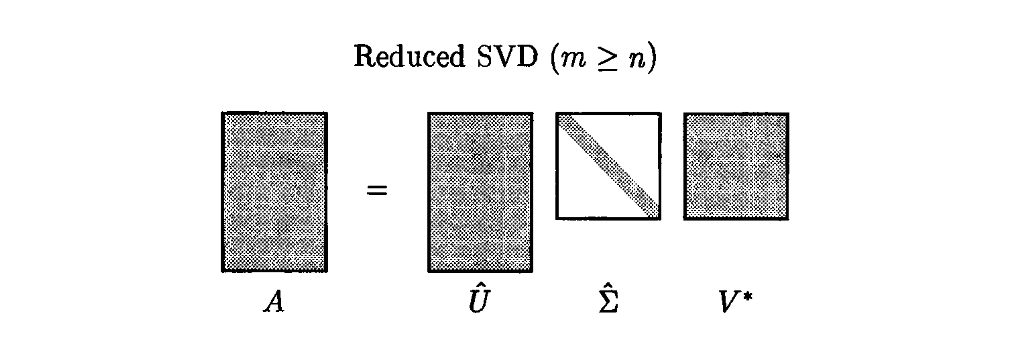
\includegraphics[width=0.8\textwidth]{figures/4-2.png}
\end{figure}
%────────────────────────────────────────

\section{Full SVD}
If we extend $U$ to a unitary matrix with extra orthonormal column vectors, we will get the full SVD. 
\begin{align*}
    A=U \Sigma V^*
\end{align*}
Here $U$ is $m \times m$ and unitary, $V$ is $n \times n$ and unitary, and $\Sigma$ is $m \times n$ and diagonal with positive real entries. Schematically:
%────────────────────────────────────────
\begin{figure}[H]
    \centering
    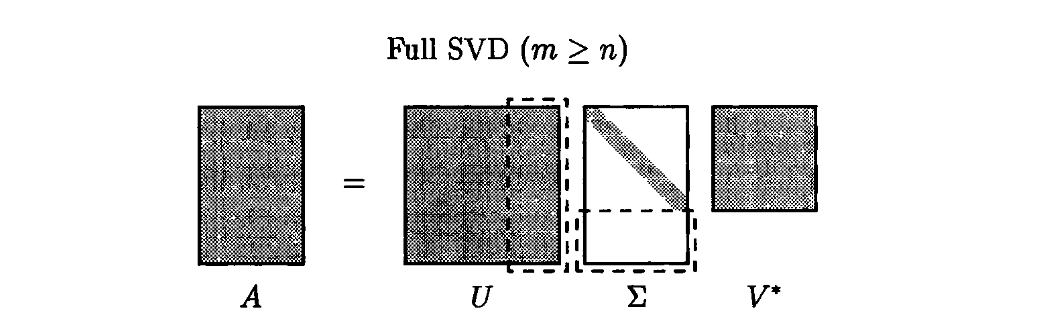
\includegraphics[width=0.8\textwidth]{figures/4-3.png}
\end{figure}
%────────────────────────────────────────

\section{Formal Definition} 
Let $m$ and $n$ be arbitrary; we do not require $m \geq n$. Given $A \in \mathbb{C}^{m \times n}$, not necessarily of full rank, a singular value decomposition (SVD) of $A$ is a factorization
\begin{align}
    \label{eq: SVD}
A=U \Sigma V^*
\end{align}
where
$U \in \mathbb{C}^{m \times m}$ is unitary,
$V \in \mathbb{C}^{n \times n}$ is unitary,
$\Sigma \in \mathbb{R}^{m \times n}$ is diagonal.
In addition, it is assumed that the diagonal entries $\sigma_j$ of $\Sigma$ are nonnegative and in nonincreasing order; that is, $\sigma_1 \geq \sigma_2 \geq \cdots \geq \sigma_p \geq 0$, where $p=\min (m, n)$.

\section{Existence and Uniqueness} 

%────────────────────────────────────────
\begin{theorem}
[Existence and uniqueness of SVD]
\label{thm: Existence and uniqueness of SVD}
Every matrix $A \in \mathbb{C}^{m \times n}$ has a singular value decomposition \eqref{eq:SVD}. Furthermore, the singular values $\left\{\sigma_j\right\}$ are uniquely determined, and, if $A$ is square and the $\sigma_j$ are distinct, the left and right singular vectors $\left\{u_j\right\}$ and $\left\{v_j\right\}$ are uniquely determined up to complex signs (i.e., complex scalar factors of absolute value 1).
\end{theorem}
%────────────────────────────────────────
%────────────────────────────────────────
\begin{proof}
\begin{itemize}
    \item Existence: Consider $\|A\|_2$ and the corresponding vector. 
    \item Uniqueness: The same. 
\end{itemize}
\end{proof}
%────────────────────────────────────────